\chapter{Исследование возможностей моделирования сетей и измерения
  сетевых характеристик в Mininet}

\section{Mininet}

\subsection{Общие сведения}

Mininet \cite{mininet} --- это виртуальная среда, которая
позволяет разрабатывать и тестировать сетевые инструменты и
протоколы. В сетях Mininet работают реальные сетевые приложения
Unix/Linux, а также реальное ядро Linux и сетевой стек. С помощью
одной команды Mininet может создать виртуальную сеть на любом типе
машины, будь то виртуальная машина, размещенная в облаке или же
собственный персональный компьютер.  Это дает значительные плюсы при
тестировании работоспособности протоколов или сетевых программ:
\begin{itemize}
\item позволяет быстро создавать прототипы программно-определяемых
  сетей;
\item тестирование не требует экспериментов в реальной сетевой среде,
  вследствие чего разработка ведется быстрее;
\item тестирование в сложных сетевых топологиях обходится без
  необходимости покупать дорогое оборудование;
\item виртуальный эксперимент приближен к реальному, так как Mininet
  запускает код на реальном ядре Linux;
\item позволяет работать нескольким разработчикам в одной топологией
  независимо.
\end{itemize}

Машины (хосты) в сети создаются по образу машины, которая запускает
Mininet, со всеми вытекающими обстоятельствами. Например, если
количество памяти, допустимое для буфера передачи сокета TCP, на
рабочей машине равно, например, значению 4096MB, то и на виртуальной
машине это значение будет таким же. Изменение конфигурации на машине в
виртуальной сети не вносит изменений в конфигурацию рабочей машины.

\subsection{Создание простой сети с помощью Python и модуля
  Mininet}

Mininet предоставляет гибкий API \cite{mininet_api} в виде модуля
для программ на языке программирования Python. С его помощью можно
строить сети различных топологий и производить с ними требуемые
манипуляции. Для того, чтобы получить доступ к API, требуется с помощью
pip \cite{pip} установить mininet и подключить данный модуль к
исполняемому файлу. Приведем пример построения сети простой топологии.
Пусть, у нас имеется 10 хостов, соединенных между собой с помощью 1
коммутатора. Нам требуется присвоить каждому ip-адрес и проверить
достижимость к каждому узлу.

Код такой программы на языке программирования Python представлен ниже:

\begin{minted}[breaklines,frame=lines,linenos,framesep=2mm,baselinestretch=1.2,fontsize=\footnotesize]{python}
from mininet.link import TCLink
from mininet.net import Mininet
from mininet.node import CPULimitedHost
from mininet.topo import Topo

'''
Создание простой топологии:
10 хостов, 1 коммутатор, 10 соединений
'''
class CustomTopology(Topo):
    def __init__(self, **opts):
        super(CustomTopology, self).__init__(**opts)
        s1 = self.addSwitch(name="s1")
        for i in range(1, 11):
            host = self.addHost(name="h%d" % i, ip="10.0.0.%d" % i)
            self.addLink(host, s1)
'''
Запуск сети и проверка достижимости элементов
'''
if __name__ == "__main__":
    topology = CustomTopology()
    net = Mininet(topo=topology, host=CPULimitedHost, link=TCLink)
    net.start()
    print("Сеть заработала")
    net.pingAll()
    net.stop()
    print("Сеть остановилась")
\end{minted}

Для того, чтобы Mininet мог знать, какую сеть строить, создается класс
топологии CustomTopology, являющийся наследником класс Topo,
предоставляемого модулем Mininet. Далее все просто: к топологии
добавляется коммутатор, через цикл добавляются хосты и соединяются с
коммутатором. В основной части программы создается объект класса
Mininet, в который мы через параметр конструктора добавляем нашу
топологию, запускаем сеть, с помощью метода Mininet \textbf{pingAll}
проверяем доступность узлов сети и, в конце концов, останавливаем сеть.

Запустим программу с помощью команды

\begin{minted}[breaklines]{bash}
  sudo python3.8 main.py 
\end{minted}

На рис.~\ref{fig:00001} видно, что все узлы являются достижимыми.

\begin{figure}[!h]
\centering
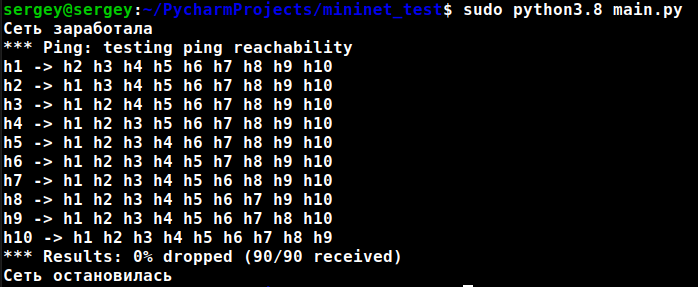
\includegraphics[width=0.7\textwidth]{image/net_start.png}
\caption{Запуск простой сети и проверка достижимости узлов}
\label{fig:00001}
\end{figure}

\subsection{MiniEdit}

Mininet предоставляет графический интерфейс управления виртуальной
сетью. MiniEdit~--- программа, написанная на языке
программирования Python, которая является надстройкой над \verb|mn| и
позволяет управлять сетью в удобном для пользователя виде. Данная
программа расположена в директории \verb|examples| исходных файлов mininet. В
моем случае это директория
\url{/usr/local/lib/python3.8/dist-packages/mininet/examples/miniedit.py}.

Создадим простую топологию из двух хостов и коммутатора в MiniEdit.

\begin{enumerate}
%\def\labelenumi{\arabic{enumi}.}
%\tightlist
\item Запустим Miniedit: % из директории
  % \url{/usr/local/lib/python3.8/dist-packages/mininet/examples/miniedit.py}.


\begin{minted}[breaklines]{bash}
  sudo python3 /usr/local/lib/python3.8/dist-packages/mininet/examples/miniedit.py
\end{minted}

\item Создадим 2 хоста, выбрав иконку терминала и кликнув по рабочей
  области 2 раза. Имена для хостов присваиваются автоматически.
\item Кликнув правой кнопкой мыши по хосту и выбрав раздел Properties,
  зададим в поле IP Adress адреса 10.0.0.1 и 10.0.0.2 соответственно
  (рис.~\ref{fig:0003}).


\begin{figure}[!h]
\centering
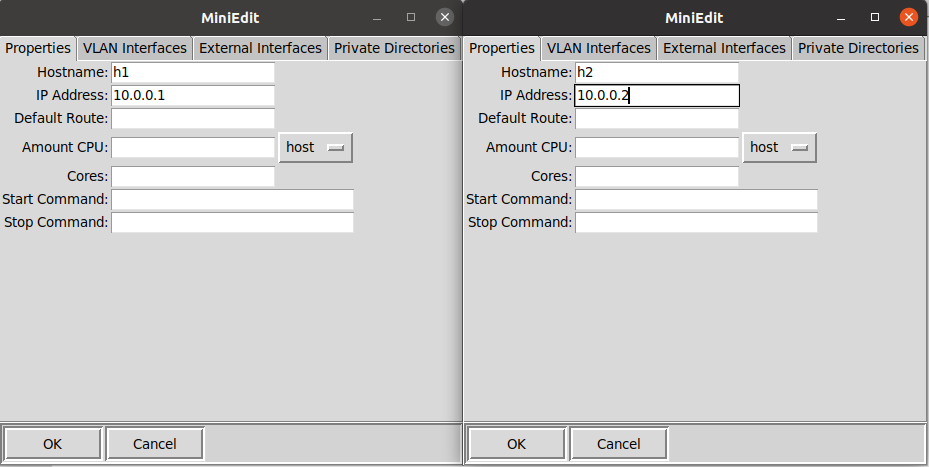
\includegraphics[width=0.8\textwidth]{image/mininet_2.3.png}
\caption{Редактирование конфигурации хостов сети}
\label{fig:0003}
\end{figure}


\item Добавим в рабочую область коммутатор, выбрав элемент
  LegacySwitch.
\item Выберем элемент NetLink и соединим элементы сети (рис.~\ref{fig:0004}).


\begin{figure}[!h]
\centering
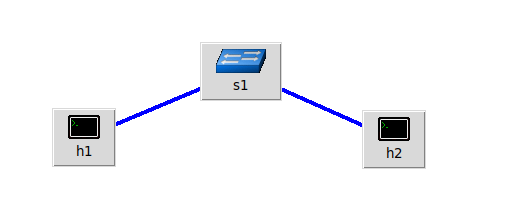
\includegraphics[width=0.5\textwidth]{image/mininet_2.4.png}
\caption{Соединение элементов сети}
\label{fig:0004}
\end{figure}


\item Запустим сеть нажав на кнопку Run.
\item Откроем терминал первого хоста, нажав правой кнопкой мыши по
  хосту и выбрав пункт Terminal. Отправим ping второму хосту (рис.~\ref{fig:0005}).

\begin{figure}[!h]
\centering
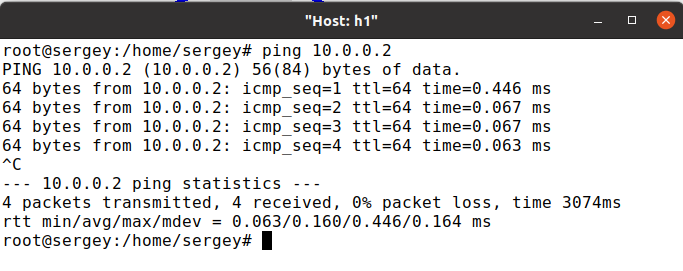
\includegraphics[width=0.6\textwidth]{image/mininet_2.5.png}
\caption{Проверка достижимости h2 для h1}
\label{fig:0005}
\end{figure}

\end{enumerate}

\section{Генерация и измерение сетевого трафика с помощью утилиты
  iPerf3}

\subsection{Общие сведения}

iPerf3 \cite{iperf} --- кроссплатформенная консольная клиент-серверная
программа-генератор TCP, UDP и SCTP трафика для тестирования
пропускной способности сети. По умолчанию тест выполняется в
направлении от клиента к серверу. Для выполнения тестирования
программа должна быть запущена на двух устройствах (это могут быть как
компьютеры, так и смартфоны, планшеты). Одно из них будет выполнять
роль сервера, а другое~--- роль клиента. Между ними и будет
происходить передача данных для измерения пропускной способности
соединения.

\subsection{Тестирование пропускной способности с помощью iPerf3}

Для запуска сервера iPerf требуется выполнить следующую команду:
\begin{minted}[breaklines]{bash}
  iperf3 -s [параметры]
\end{minted}

Для запуска iPerf-клиента требуется выполнить следующую команду:
\begin{minted}[breaklines]{bash}
  iperf3 -c server_ip [параметры]
\end{minted}

Подробнее со списком параметров iPerf3 можно ознакомиться
в~\cite{iperf_userdoc}.

Проведем тестирование сети в Mininet:
\begin{enumerate}
%\def\labelenumi{\arabic{enumi}.}
%\tightlist
\item Запустим MiniEdit.
\item Создадим 2 хоста (h1 и h2) и коммутатор (s1).
\item Соединим элементы сети.
\item Запустим сеть (рис.~\ref{fig:0011}).


\begin{figure}[!h]
\centering
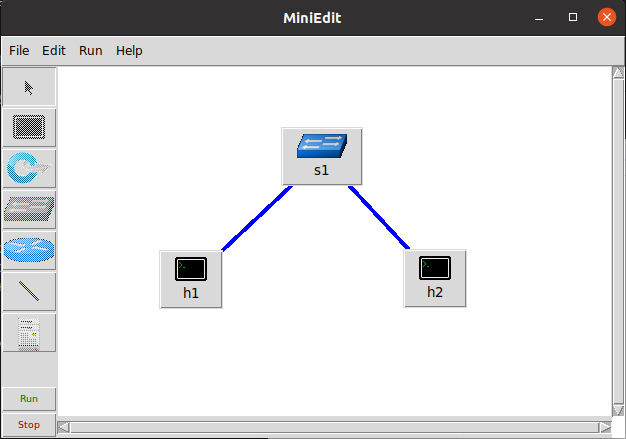
\includegraphics[width=0.8\textwidth]{image/iperf_1.png}
\caption{Сеть с простой топологией в Mininet}
\label{fig:0011}
\end{figure}

\item Запустим iPerf-сервер на h2.
\begin{minted}[breaklines]{bash}
  iper3 -s
\end{minted}

\item Запустим iPerf-клиент на хосте h1 на 60 секунд, пропустив первые
  10 секунд для статистики (рис.~\ref{fig:0012}):
\begin{minted}[breaklines]{bash}
  iperf3 -c 10.0.0.2 -t 60 -O 10
\end{minted}

\begin{figure}[!h]
\centering
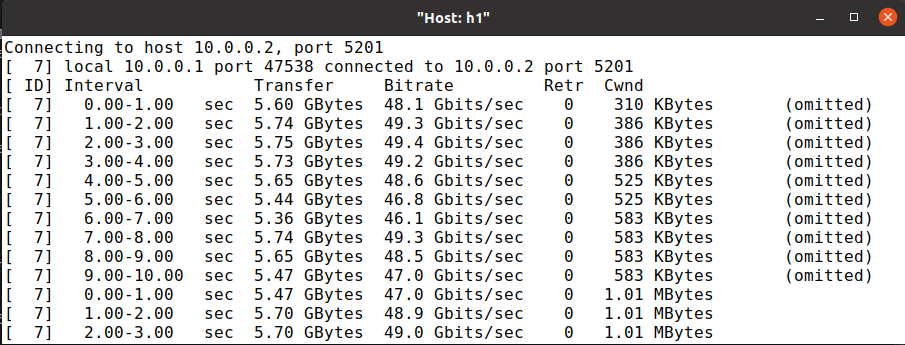
\includegraphics[width=0.8\textwidth]{image/iperf_3.png}
\caption{Запуск iPerf-клиента}
\label{fig:0012}
\end{figure}


\item Просмотрим статистику, которую сгенерировал iPerf
  (рис.~\ref{fig:0013}).

\begin{figure}[!h]
\centering
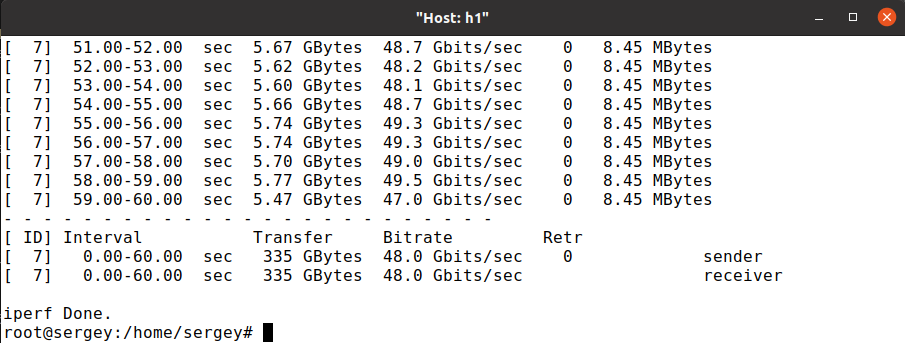
\includegraphics[width=0.8\textwidth]{image/iperf_4.png}
\caption{Вывод статистики iPerf3}
\label{fig:0013}
\end{figure}

\end{enumerate}

\section{Использование утилиты iproute2 для настройки интерфейсов
  сетевых элементов}

\subsection{Общие сведения}

Iproute2 \cite{iproute} --- это набор утилит для управления
параметрами сетевых устройств в ядре Linux. Эти утилиты были
разработаны в качестве унифицированного интерфейса к ядру Linux,
которое непосредственно управляет сетевым трафиком.

Iproute2 заменил полный набор классических сетевых утилит UNIX, которые
ранее использовались для настройки сетевых интерфейсов, таблиц
маршрутизации и управления ARP-таблицами: ifconfig, route, arp, netstat
и других, предназначенных для создания IP-туннелей. Iproute2 предлагает
унифицированный синтаксис для управления самыми разными аспектами
сетевых интерфейсов.

Набор утилит включает в себя три основные программы:
\begin{itemize}
\item ip \cite{ip} --- утилита для просмотра параметров и
  конфигурирования сетевых интерфейсов, сетевых адресов, таблиц
  маршрутизации, правил маршрутизации, ARP-таблиц, IP-туннелей,
  адресов multicast-рассылки, маршрутизацией multicast-пакетов;
\item tc \cite{tc} --- утилита для просмотра и конфигурирования
  параметров управления трафиком, позволяющая управлять классификацией
  трафика, дисциплинами управления очередями для различных классов
  трафика либо целиком для сетевого интерфейса, что, в свою очередь,
  позволяет реализовать QoS в нужном для системы объёме:
  \begin{itemize}
  \item разделение разных типов трафика по классам;
  \item назначение разных дисциплин обработки очередей трафика с
    разным приоритетом, механизмами прохождения очереди, ограничениями
    по скорости и т.\,п.;
  \end{itemize}
\item ss \cite{ss} --- утилита для просмотра текущих соединений и
  открытых портов, является аналогом утилиты netstat.
\end{itemize}

\subsection{Утилита tc}

Утилита tc \cite{tc} наиболее полезна для исследования, так
как она позволяет гибко настроить поведение контроля исходящего трафика.

Система контроля трафика состоит из следующих компонентов:
\begin{itemize}
\item \textbf{Ограничитель исходящего трафика}. Когда трафик
  сформирован, его полоса пропускания начинает
  контролироваться. Ограничение может дать больше, чем уменьшение
  полосы пропускания --- оно также используется для сглаживания пиков
  для более прогнозируемого поведения сети.
\item \textbf{Планировщик передачи пакетов}. Механизм позволяет
  увеличить интерактивность исходящего трафика при гарантировании
  полосы пропускания для передачи данных большого объема. Такое
  упорядочение также называется приоритезацией и применяется для
  исходящего трафика.
\item \textbf{Ограничитель исходящего трафика}. Этот механизм
  позволяет ограничить количество пакетов или байт в потоке входящего
  трафика, соответствующих определенной классификации.
\item
  \textbf{Отбрасыватель}. Трафик, превышающий установленную полосу
  пропускания, может быть отброшен как для входящего, так и исходящего
  трафика. Обработка трафика контролируется тремя типами объектов:
  очередями, классами и фильтрами. 
\end{itemize}

Для получения информации о tc используется команда
\begin{minted}[breaklines]{bash}
  tc help
\end{minted}

Дисциплина очереди --- это алгоритм обработки очереди сетевых пакетов.
Дисциплин на одном интерфейсе может быть задействовано несколько, а
непосредственно к интерфейсу прикрепляется корневая дисциплина (root qdisc).
При этом каждый интерфейс имеет свою собственную корневую дисциплину.
Каждой дисциплине и каждому классу назначается уникальный дескриптор,
который может использоваться последующими инструкциями для ссылки на эти
дисциплины и классы. Помимо исходящей дисциплины интерфейс так же может
иметь и входящую дисциплину, которая производит управление входящим
трафиком. Дисциплины на интерфейсе образуют иерархию, где вверху
иерархии находится корневая дисциплина. Сам интерфейс ничего не знает о
дисциплинах, находящихся под корневой, а поэтому работает только с ней.
Дисциплины делятся на классовые (CBF, HTB, PRIO) и бесклассовые (pfifo,
pfifo\_fast, RED, SFQ, TBF). Подробнее о видах дисциплин очередей можно
прочесть в~\cite{tc}.

Воспользуемся сетью Mininet и с помощью tc выведем информацию о
дисциплине очереди на сетевом устройстве s1-eth0 (интерфейс
коммутатора, к которому подключен хост h1). Для этого воспользуемся
командой
\begin{minted}[breaklines]{bash}
  tc -s qdisc show dev s1-eth1
\end{minted}

На рис. \ref{fig:0020} видно, что корневой дисциплиной очереди назначена
дисциплина noqueue. Данная дисциплина означает «отправляй мгновенно, не
ставь в очередь».


В выводе tc можно увидеть полезные для исследования данные:
\begin{itemize}
\item \emph{Sent 0 bytes 0 pkt (dropped 0, overlimits 0 requeues
    0)}~--- означает, что было отправлено 0 байт (0 пакетов), из
  которых 0 пакетов отброшено и 0 пакетов вышли за пределы лимита.
\item \emph{backlog 0b 0p requeues 0} --- размер очереди в байтах и
  пакетах.
\end{itemize}

\begin{figure}[!h]
\centering
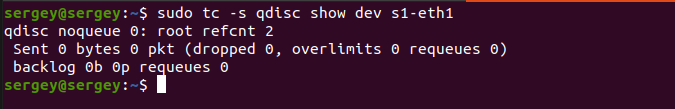
\includegraphics[width=0.9\textwidth]{image/iproute_tc_qdisc_show_s1-eth1.png}
\caption{Информация о дисциплине очереди на сетевом устройстве
  s1-eth0}
\label{fig:0020}
\end{figure}


Запомним параметр backlog~--- он будет полезен нам при сборе
статистики.
